\chapter{Einleitung}


An der HAW wurde im Rahmen des Forschungprojektes X-Multirotor Untersucht, ob in Zukunft Windkraftanlegen mit mehreren Rotoren eine Alternative zu herkömmlichen WKA darstellen könnten. Dazu wurde unter Anderem ein Modell im Labormaßstab entwickelt. Das Grundkonzept wird in \ref{fig:multirotor} verdeutlicht.

\begin{figure}[htbp] % Positionierungsoptionen: h=here, t=top, b=bottom, p=page of floats
    \centering % Zentriert das Bild
    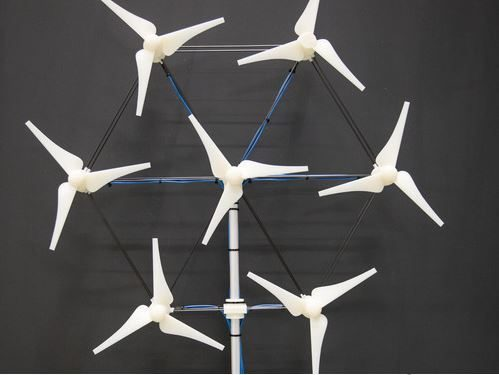
\includegraphics[width=0.8\textwidth]{figures/multirotor.jpg} % Pfad zum Bild und Skalierung
    \caption{Modell einer Multirotor-Windenergieanlage der HAW \cite{fink_multirotorjpg_2018}} % Bildunterschrift
    \label{fig:multirotor} % Label für Referenzen im Text
\end{figure}

Multirotor-Windkraftanlagen könnten signifikante Vorteile gegenüber konventionellen Anlagen bieten. Einer der Hauptvorteile ist die reduzierte Masse im Vergleich zu herkömmlichen Turbinen. Durch die Verwendung mehrerer kleinerer Rotoren wird die Gesamtmasse der Struktur verringert, was zu effizienteren und kostengünstigeren Konstruktionen führt \cite{jamieson_multi-rotors_2012}. Ein weiterer Vorteil ist die erhöhte Zuverlässigkeit durch unabhängige Rotoren. Im Falle eines Ausfalls muss nicht die gesamte Anlage stillgelegt werden, sondern nur der betroffene Rotor, was die Verfügbarkeit der Anlage erhöht.Darüber hinaus ermöglicht die große Stückzahl der Rotorblätter in Multirotor-Systemen eine intensivere Optimierung des Designs und der Fertigungsprozesse, was zu erheblichen Kostensenkungen führen kann.

Um das Verhalten und die Steuerungsmöglichkeiten einer MRWT weiter zu untersuchen, soll ein Demonstrator im Labormaßstab genutzt werden. Dieser Demonstrator wurde bereits entwickelt und gebaut. Die Entwicklung der Rotorblätter (Rotordurchmesser 450mm) erwies sich aufgrund der ungewöhnlichen Betriebsbedingungen und Fertigungsschwierigkeiten allerdings als schwierig. Die aktuell verwendeten Rotorblätter erwiesen sich in Windkanaltests als nicht leistungsfähig genug. Ziel der vorliegenden Arbeit ist es, ein verbessertes Rotorblatt zu entwerfen und zu testen.
\section{Anforderungen und Randbedingungen}
Um mit dem bestehenden Demonstrator optimal funktionieren zu können, wurden in \cite{buchholz_erarbeitung_2020} einige Randbedingungen für den Betrieb der Rotorblätter festgelegt:
\begin{itemize}
    \item Art der Leistungsregelung: Pitch, Variation der elektrischen Last
    \item Schnelllaufzahl: 7
    \item Windbereich: 2-15 m/s
    \item Optimierung für 6-8 m/s
    \item Rotordurchmesser: 450 mm
    \item Generator Drehzahl: max. 5500 1/min
    \item Generator Drehzahl: max. 5500 1/min
    \item Generator Drehmoment: opt. 130 mNm, max. 250 mNm
\end{itemize}

Die physische Schnittstelle zwischen Rotorblatt und Generator wird als Teil dieser Arbeit näher betrachtet und überarbeitet.

Für die Erprobung des Multirotor-Demonstrators wird eine Vielzahl von Einzelrotoren mit entsprechend vielen Rotorblättern benötigt. Daher sollen die Rotorblätter möglichst einfach und günstig in einem Kleinserienprozess gefertigt werden können.

\section{Vorarbeit und Probleme}
Die bisherigen Bemühungen, ein geeignetes Rotorblatt zu finden, verteilen sich auf drei Masterprojekte: Zuerst wurde in \cite{buchholz_erarbeitung_2020} auf Basis aerodynamischer Profile aus Literaturquellen ein optimiertes Rotorblattdesign entwickelt. Für dieses Rotorblattdesign sollte in \cite{stolla_konstruktion_2020} ein geeignetes Fertigungsverfahren gefunden und getestet werden. Aufgrund der sehr filigranen Geometrie (Profiliefe ca. 10mm, Dicke < 1mm) scheiterten die Versuche, das Blatt herzustellen. Daraufhin entschieden die Projektverantwortlichen, ein geändertes Rotorblattdesign mit einem dickeren Profil im FDM Druckverfahren zu fertigen und zu testen. Die Tests wurden durch \textcite{loof_windkanaluntersuchungen_2023} durchgeführt. Der beste ermittelte Leistungsbeiwert liegt unter den Erwartungen. Als Hauptursache vermutete das Team des CC4E die Auslegung der Rotorblätter. Dies ging aus Gesprächen mit Prof. Peter Dalhoff und der Aufgabenstellung hervor.

\textcite{buchholz_erarbeitung_2020} fanden während der ersten Blattauslegung Anzeichen dafür, dass dünne gebogene Platten im relevanten Re-Bereich bessere Ergebnisse liefern könnten. Auch \textcite{liu_optimization_2014} und \textcite{bastankhah_new_2017} stützen diese Vermutung.

\section{Lösungsansatz}
Um ein besseres Blatt bei gleichzeitig verbesserter Herstellbarkeit zu entwerfen, werden Profile konstanter Dicke mit modifizierten Vorder-und Hinterkanten näher untersucht. Um die bestmögliche Form zu finden, soll eine Optimierungsstudie durchgeführt werden. Gemäß bewährten aerodynamsichen Theorien zur Rotorblattauslegung sollen die optimale Blattverwindung und Profiltiefenverteilung für das optimierte Profil festgelegt werden. Das Ergebnis ist auf ausreichende Festigkeit zu prüfen, bevor es gefertigt und im Windkanal getestet werden soll.